\documentclass[a4paper,11pt]{article}
\usepackage{amssymb}
\usepackage{latexsym}
\usepackage{eufrak}
\usepackage{euscript}
\usepackage{exscale}
\usepackage{graphicx}
\usepackage{mathrsfs}
\usepackage{epsfig}
\usepackage{hyperref}
\usepackage{adjustbox}

\usepackage[hypcap]{caption}
\usepackage{fancyhdr}
\usepackage[german]{babel}
\usepackage[latin1,utf8]{inputenc}
\usepackage{pdfpages}
\usepackage{amsthm}
\usepackage{color}
\usepackage{listings}
\usepackage{float}
\usepackage{titlesec}



\lstset{
basicstyle=\scriptsize\tt,
}

\lstset{ %
  language=R,                     % the language of the code
  basicstyle=\footnotesize,       % the size of the fonts that are used for the code
  numbers=left,                   % where to put the line-numbers
  numberstyle=\tiny\color{gray},  % the style that is used for the line-numbers
  stepnumber=1,                   % the step between two line-numbers. If it's 1, each line
                                  % will be numbered
  %firstnumber=\numexpr\inputlineno+1\relax
  numbersep=5pt,                  % how far the line-numbers are from the code
  %backgroundcolor=\color{white},  % choose the background color. You must add \usepackage{color}
  showspaces=false,               % show spaces adding particular underscores
  showstringspaces=false,         % underline spaces within strings
  showtabs=false,                 % show tabs within strings adding particular underscores
  %frame=single,                   % adds a frame around the code
  rulecolor=\color{black},        % if not set, the frame-color may be changed on line-breaks within not-black text (e.g. commens (green here))
  tabsize=1,                      % sets default tabsize to 2 spaces
  captionpos=NA,                   % sets the caption-position to bottom
  breaklines=true,                % sets automatic line breaking
  breakatwhitespace=false,        % sets if automatic breaks should only happen at whitespace
  title=\lstname,                 % show the filename of files included with \lstinputlisting;
                                  % also try caption instead of title
  keywordstyle=\color{blue},      % keyword style
%  commentstyle=\color{dkgreen},   % comment style
  %stringstyle=\color{red},      % string literal style
  escapeinside={\%*}{*)},         % if you want to add a comment within your code
  morekeywords={*,...}            % if you want to add more keywords to the set
} 


\pagestyle{fancy}
%\pagenumbering{arabic}
%\rhead{\small{\today}}
\chead{}
\lhead{\small{Statistics, Visualization and more using R}}
\rhead{Bradley Mackay, Clemens Ehlich}
\rfoot{\small{\textcolor{gray}{clemens.ehlich@sbg.ac.at}}}
\lfoot{\small{\textcolor{gray}{Master Data Science @Universität Salzburg 
}}}
\renewcommand{\headrulewidth}{0.4pt}
\renewcommand{\footrulewidth}{1pt}
\setlength{\headwidth}{420pt}
\newcommand{\sectionbreak}{\clearpage}

\markright{}


\setlength{\textheight}{665pt}
\setlength{\textwidth}{440pt}
\setlength{\marginparwidth} {10pt}
\setlength{\hoffset}{-30pt}
\setlength{\voffset}{-50pt}
\fancyhfoffset[R]{0.5mm} 
\setlength{\headsep}{1cm}

\newtheorem{defin}{Definition}[section]
\newtheorem{satz}[defin]{Theorem}
\newtheorem{folg}[defin]{Proposition}
\newtheorem{bem}[defin]{Bemerkung}
\newtheorem{lem}[defin]{Lemma}
\newtheorem{hs}[defin]{Lemma}
\newtheorem*{remark}{Bemerkung}



\hyphenation{bio-mim-ic-ry bio-in-spi-ra-tion re-us-a-ble pro-vid-er ha-ving con-si-de-ring
 cor-res-pon-ding}

\begin{document}
\hrule
\begin{center}
\Large{\textbf{Statistics, Visualization and more using R}} \\[3mm]
\hrule
\hrule 
\vspace{2mm}
\LARGE{\textbf{R Packages: A Beginner's Guide }} \\[2mm] 
\hrule
\hrule
\vspace{6mm}
\large{ \textbf{Bradley Mackay, Clemens Ehlich}	
}\\[5mm]

\end{center}
\begin{center}
\today
\end{center}
\hrule
\vspace{3cm}


\begin{center}
\large{\textbf{Summary}}
\end{center}
One of the biggest advantages of the R programming language is the existence of an unbelievable number of extension packages, which make your daily work much easier. R packages are collections of functions and datasets and are mostly created by the community itself. As the title suggests, this short paper is about how to create your own little R package, because creating your own package has many advantages. Especially if you have to work on recurring tasks. For this we will first give a summary of important commands to work with packages. Then we will give an overview how packages are built and finally we will give a step by step guide how to create your first own package.
\\
\\
\\
\begin{center}
	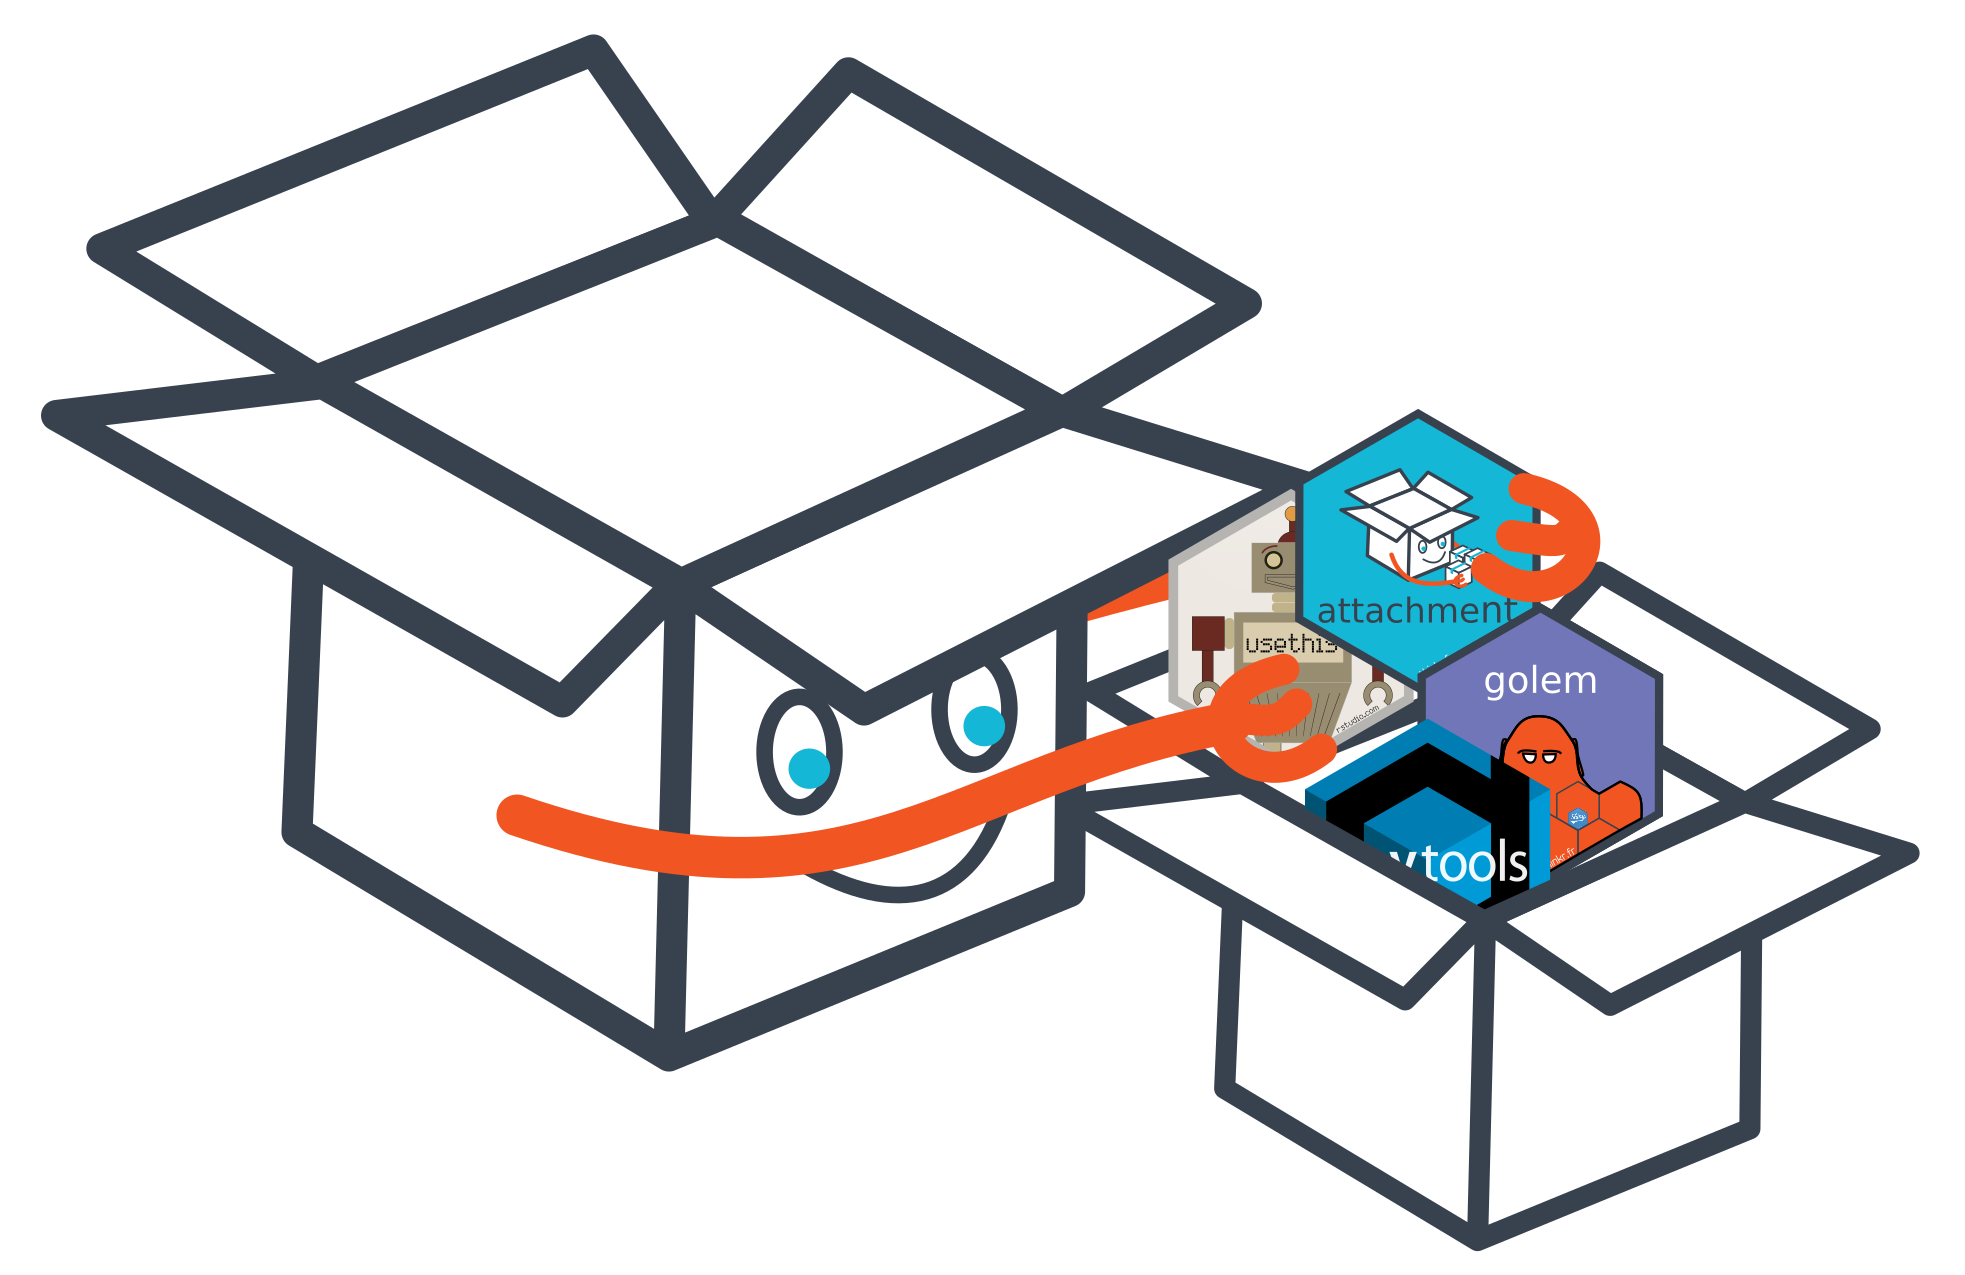
\includegraphics[width=0.6\linewidth]{pack}
\end{center}  

\tableofcontents
\vspace*{2cm}
\clearpage

\section{Basics}
\subsection{What's a package}

As already mentioned at the beginning R packages are collections of functions and data sets. They extend the basic functionalities of the Language itself or add new ones. The packages can be written in R code, but for example also in C++ (with the rcpp-package). But at the beginning you should concentrate on the Rcode variant.

\subsection{Why Packages?}
To use foreign packages, makes your workflow a lot easier and faster. Because for  recurring tasks its not necessary to reinvent the wheel again and again. There are more than 19.000 packages on CRAN. For nearly every common Problem a package exist, for example to load or visualize data. Packages form also interfaces to other software and their file formats (foreign, caffe, RQGIS,...), databases (RODBC, RPostgreSQL,...), other programming languages (Rcpp, RPython,...) or webservices (Rfacebook, RGoogleAnalytics,...).

\subsection{Where can i find packages?}

To get an overview, which packages are already available its good to use the website \textit{https://www.rdocumentation.org/}. It list nearly every Package which official exists. You can also look at \textit{https://cran.r-project.org} the official R Website or  
BioConductor a website for Biology Content (\textit{http://bioconductor.org/}). Of course there are also countless packages on GitHub (\textit{https://github.com/}).

\subsection{Some important R-Commands to work with packages}


\begin{lstlisting}[frame=single]
# Installing Packages:
install.packages("xyz") 
install.packages(c("xyz", "123"))

# check and update Packages:
old.packages("xyz")
update.packages("xyz")

# remove Packages:
remove.packages("xyz")
\end{lstlisting}
There is one big problem: each repository (CRAN, BioConductor,..) has its own way to install a package from them. To simplify this process you can use the package $ "devtools" $. But for this you might also need to install $ "Rtools" $ for Windows, $ "Xcode" $ for Mac or if you using Linux $"r-devel"$ for Linux. But then you can install packages directly from the repositorys with the following code: 


\begin{lstlisting}[frame=single]
install_bioc() #from Bioconductor
install_cran() #from CRAN
install_github() #from GitHub
install_local() #from a local file
install_url() #from a URL
\end{lstlisting}

\section{Making you own Pakage}
\subsection{What does a package consist of?}
In this chapter we want to show how to create your own package. For this it is important to know how a package is built. If you create a new file to create an R-package, a folder structure is automatically created in the background. This folder structure is shown in the following figure. The DESCRIPTION-Files, the NAMESPACE, the FUNCTIONS and the MANUALS are mandatory. The rest, which is dotted in the graphic, is optional.
\\
\begin{center}
	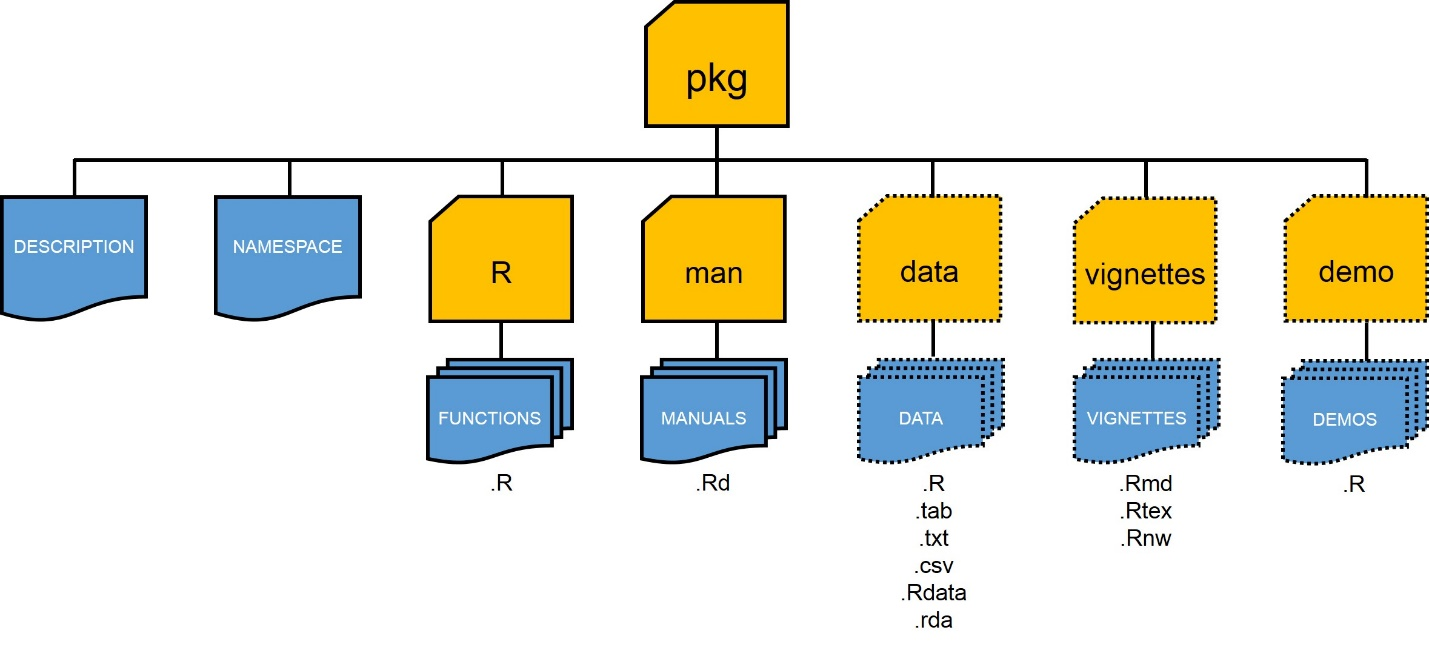
\includegraphics[width=1\linewidth]{stott}
\end{center}  




\section{Related literature}


\begin{thebibliography}{laengste Labelbreite}
   \bibitem[text]{bezugspunkt}
\end{thebibliography}


\end{document}

